\documentclass{beamer}
\beamertemplatenavigationsymbolsempty


\usepackage{microtype}
\usepackage[slovak,USenglish]{babel}
\usepackage[utf8]{inputenc}
\usepackage[T1]{fontenc}

\usepackage{amsmath}
\usepackage{tikz}
\usetikzlibrary{arrows.meta, quotes, calc}


\newcommand{\bra}[1]{\langle#1\rvert} % Bra
\newcommand{\ket}[1]{\lvert#1\rangle} % Ket
\newcommand{\qprod}[2]{ \langle #1 | #2 \rangle} %Inner Product
\newcommand{\braopket}[3]{\langle #1 | #2 | #3\rangle} % Matrix Element
\newcommand{\expect}[1]{ \langle #1 \rangle} % Expectation value
\newcommand\abs[1]{\left|#1\right|}

% Theme
\usetheme{Boadilla}

% Title page
\title{Optimalizácia variačných kvantových eigensolverov}
\author{Michal Švec}
\institute{doc. RNDr. Martin Plesch, PhD.}
\date{}

\makeatother
\setbeamertemplate{footline}
{
  \leavevmode%
  \hbox{%
  \begin{beamercolorbox}[wd=.9\paperwidth,ht=2.25ex,dp=1ex,center]{author in head/foot}%
    \usebeamerfont{author in head/foot}\insertshorttitle
  \end{beamercolorbox}%
  \begin{beamercolorbox}[wd=.1\paperwidth,ht=2.25ex,dp=1ex,center]{date in head/foot}%
    \insertframenumber{} /\inserttotalframenumber\hspace*{1ex}
  \end{beamercolorbox}}%
  \vskip0pt%
}
\makeatletter
\setbeamertemplate{navigation symbols}{}
\setbeamertemplate{itemize items}[circle]
\setbeamertemplate{caption}{\raggedright\insertcaption\par}



% Begin document
\begin{document}

% Title slide
\begin{frame}
	\titlepage
\end{frame}

\begin{frame}
	\frametitle{Variačný kvantový eigensolver (VQE)}
			
	\begin{itemize}
		\item hybridný algoritmus
		\begin {itemize}
		    \item používame štandardný a kvantový počítač
            \item na štandardnom počítači beží optimalizačný algoritmus
	    \end{itemize}
        \item hľadá najmenšie vlastné číslo matice
    \end{itemize}
    \begin{columns}[T] % align columns at the top
        \begin{column}{0.0\textwidth} % adjust the left margin
        \end{column}
        \begin{column}{0.95\textwidth} % adjust the width of the block
            \begin{tikzpicture}
                \node[draw, rectangle, minimum width = 1.5 cm, minimum height = 1.5 cm] (fl) at (0,0) {VQE};
                \node[above] at (fl.north) {};
                \draw [Triangle-] (fl.west) -- node[above]{reprezentácia problému} node[below]{parametrizovaný kvantový obvod} ++(-5.5,0);
                \draw [-Triangle] (fl.east) -- node[above]{najmenšie vlastné číslo} node[below]{} ++(4,0);
            \end{tikzpicture}
        \end{column}
    \end{columns}

    \begin{itemize}
		\item v našom prípade
		\begin{itemize}
		    \item reprezentácia problému = 4-qubitová reprezentácia molekuly vodíka 
            \item najmenšie vlastné číslo = základný stav molekuly vodíka
	    \end{itemize}
    \end{itemize}
			
\end{frame}

\begin{frame}
	\frametitle{Ciele práce}
	\begin{itemize}
		\item hľadanie najjednoduchšieho kvantového obvodu vedúceho k výsledku
        \item konvergencia energie veľmi závisí od voľby optimalizačného algoritmu
	\end{itemize}
    \begin{columns}[T] % align columns at the top
        \begin{column}{0.05\textwidth} % adjust the left margin
        \end{column}
        \begin{column}{0.9\textwidth} % adjust the width of the block
            \begin{block}{Porovnávanie výkonnosti}
                \begin{itemize}
                    \item 15 optimalizačných algoritmov a 18 parametrizovaných kvantových obvodov
                    \item 270 kombinácií $(15 * 18)$ konfigurácie VQE
                    \item každú kombináciu sme spustili 50-krát
                    \item hľadanie súvislostí vo vyprodukovaných dátach
                \end{itemize}
            \end{block}
        \end{column}
        \begin{column}{0.05\textwidth} % adjust the right margin
        \end{column}
    \end{columns}
   
	
\end{frame}

\begin{frame}
	\frametitle{Príklad konvergencie energie}
    \begin{figure}[H]
        \centering
        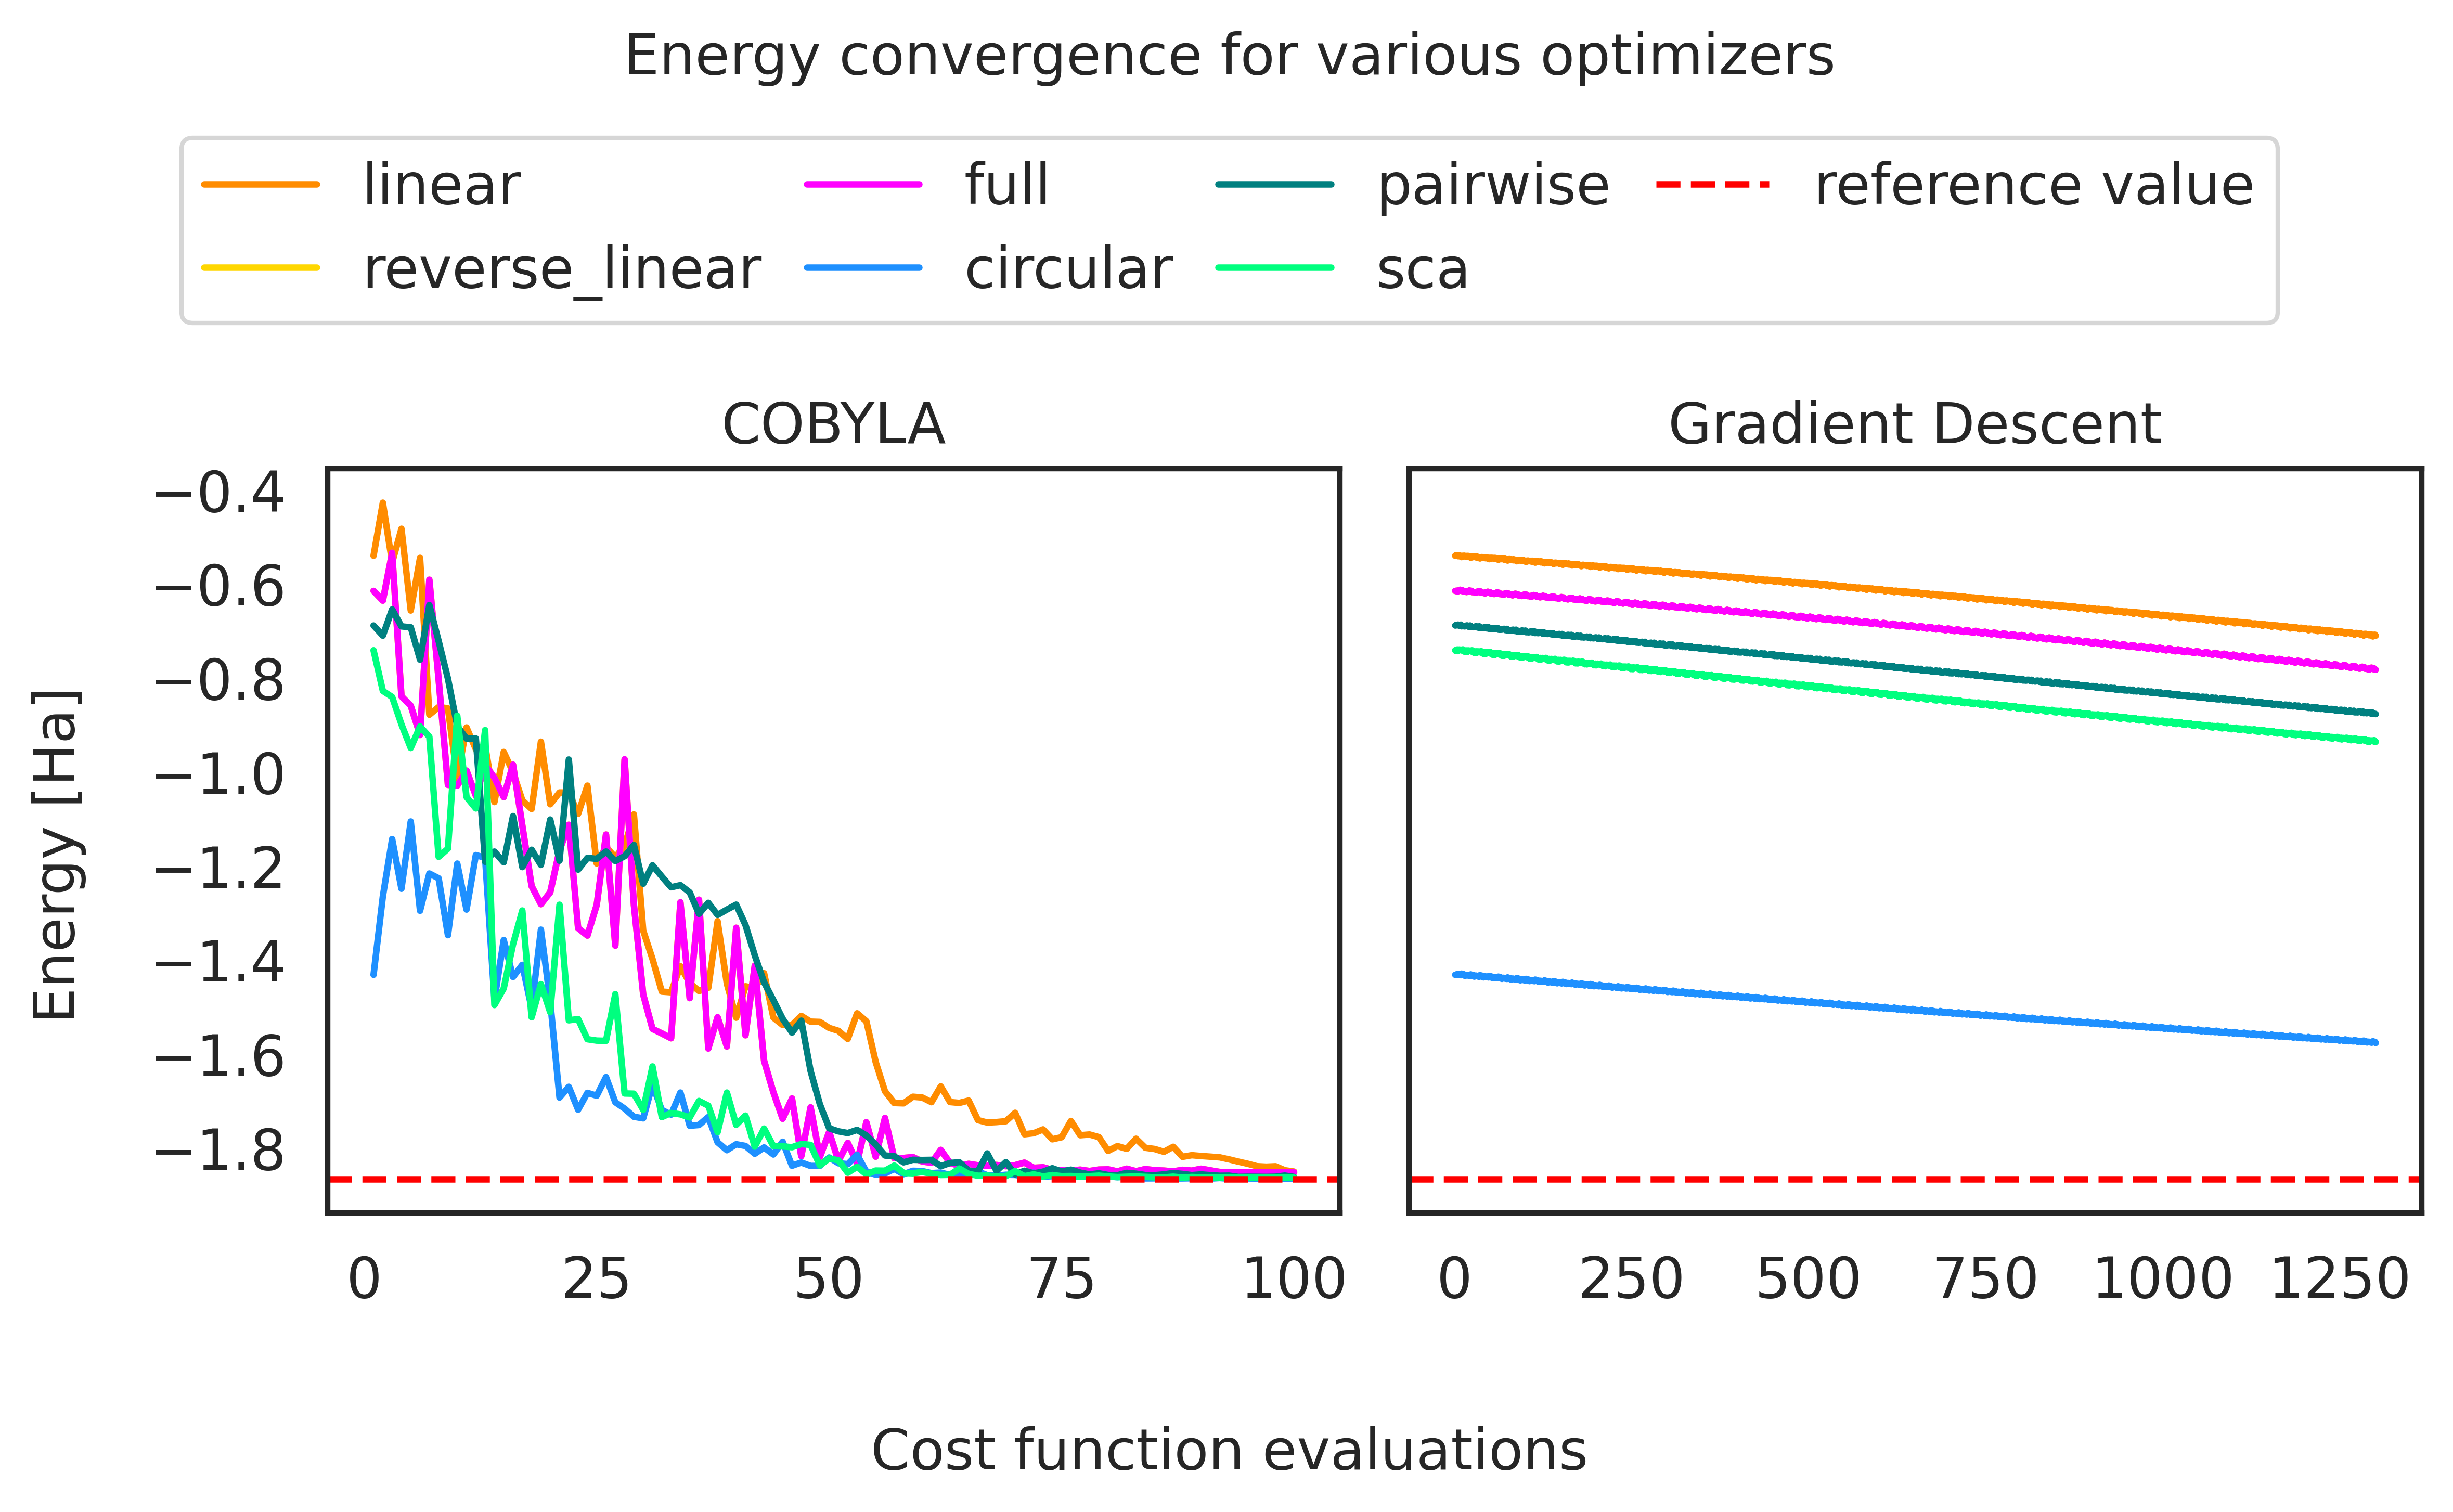
\includegraphics[width=\textwidth]{/Users/michalsvec/Desktop/3Y/bachelor_thesis/optimization-of-variational-quantum-eigensolvers/images/convergence_example.png}
    \end{figure}
\end{frame}

\begin{frame}
	\frametitle{Súčasný stav}
   
	\begin{itemize}
		\item so školiteľom sme si prešli napísanú prácu
        \item momentálne zapracovávam všetky pripomienky
        \item v podstate máme takmer hotovo
	\end{itemize}

    \begin{columns}[T] % align columns at the top
        \begin{column}{0.05\textwidth} % adjust the left margin
        \end{column}
        \begin{column}{0.9\textwidth} % adjust the width of the block
            \begin{block}{Problémy a výzvy}
                \begin{itemize}
                    \item fyzika
                    \item veľa dát
                \end{itemize}
            \end{block}
        \end{column}
        \begin{column}{0.05\textwidth} % adjust the right margin
        \end{column}
    \end{columns}
\end{frame}
\end{document}